
\chapter{Implementation}
\label{chap:implementation}


We presented the design of the system in the Design chapter
(Chapter~\ref{chap:design}).  This chapter describes how we
implemented it using Java$^{\textrm{TM}}$ Platform, Enterprise Edition
(Java EE).  After briefly introducing the key aspects of Java EE in
the Java EE Platform section (\S\ref{sec:jee}), this chapter presents
the key implentation details for each tier of the application.

\section{Java EE Platform}
\label{sec:jee}

This section introduces the readers to the elements of the Java EE
platform to develop and run this system.

\subsection{Java EE Architecture}
\label{sec:jeeintro}


...




\section{Implementation Overview}
\label{sec:implementsteps}

Figure~\ref{fig:architecture2} shows the bird's eye view of the
objects in this system. There are three distinct tiers: presentation,
business, and entity.

...


\begin{landscape}
\begin{figure}[!htpb] 
  \centering
  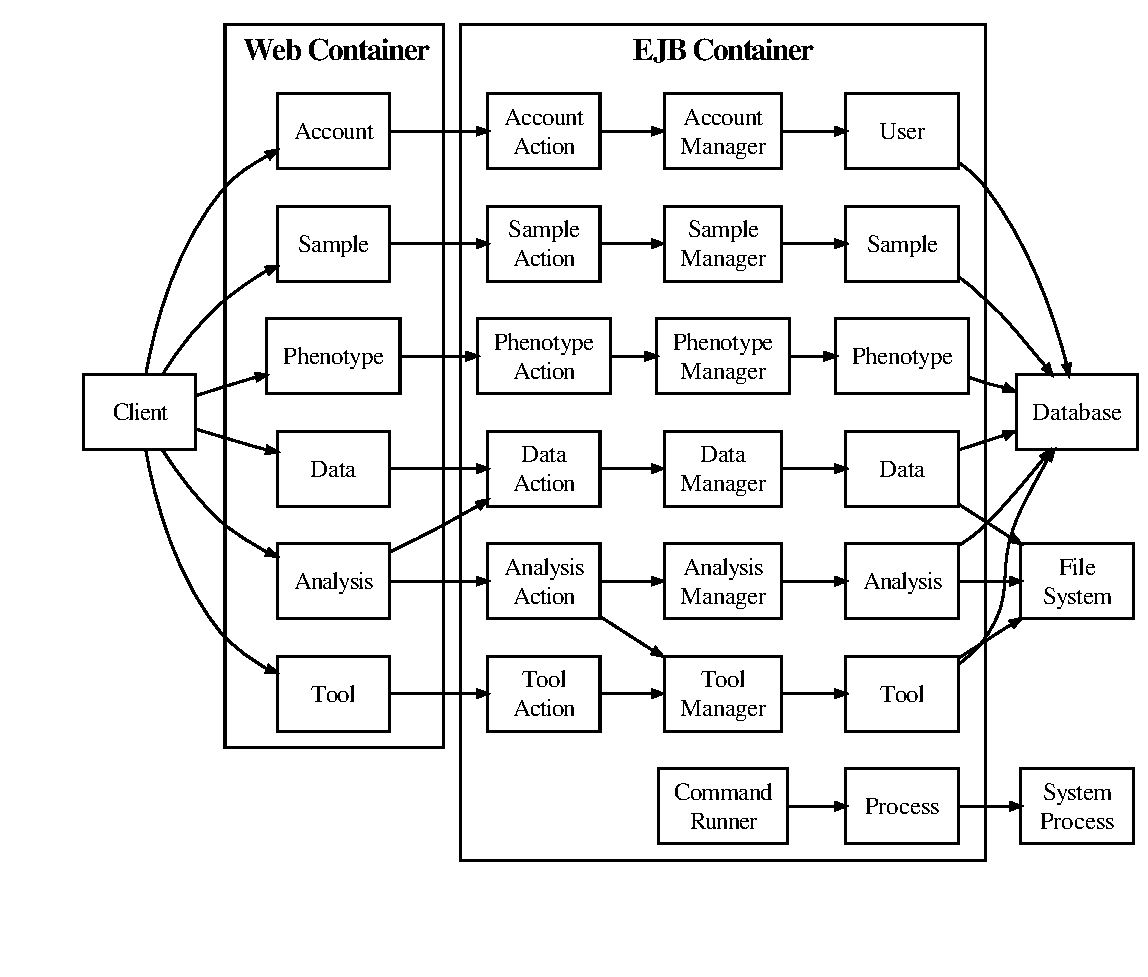
\includegraphics[width=1.1\textwidth]{diagrams/Architecture2}
%  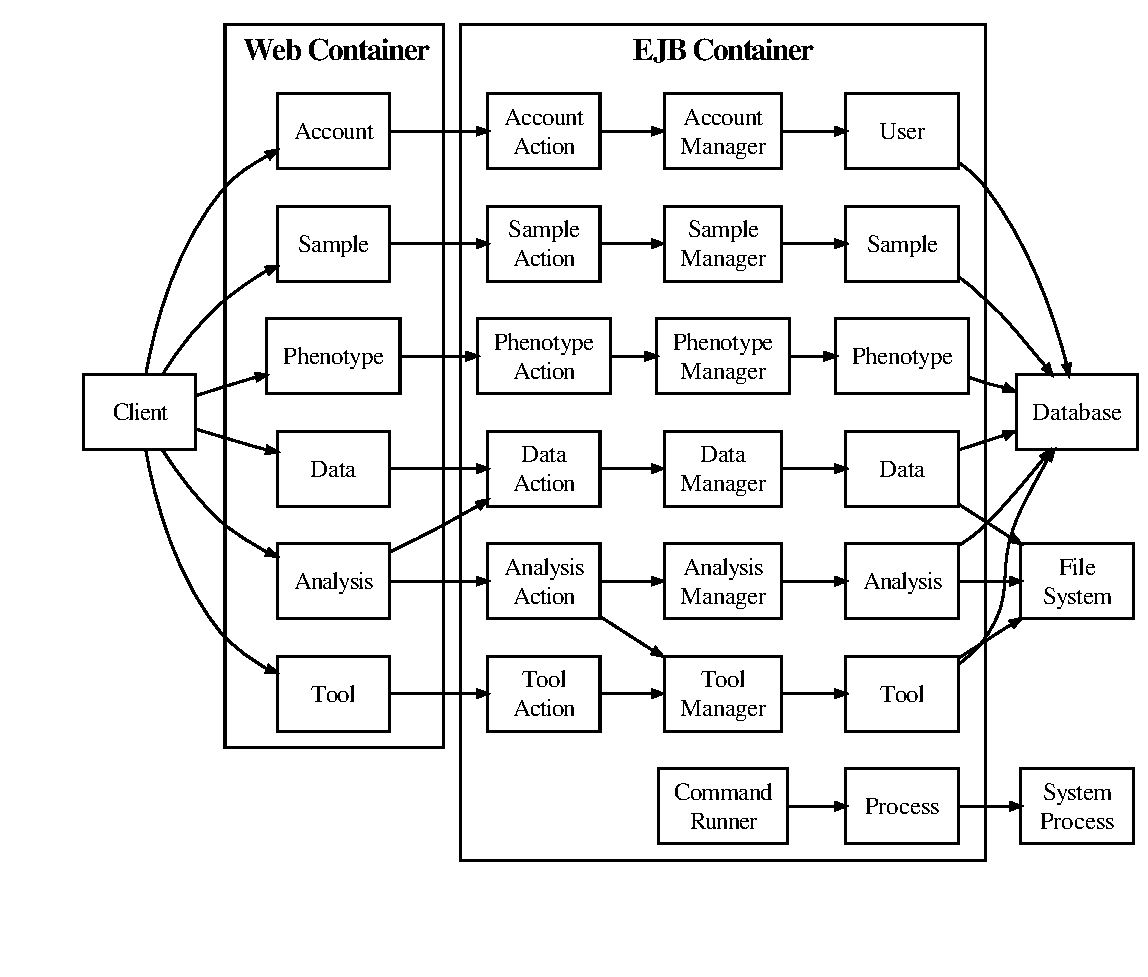
\includegraphics[height=.8\textheight]{diagrams/Architecture2.pdf}
  \caption{High-level object view of the system}
  \label{fig:architecture2}
\end{figure}
\end{landscape}





\section{Presentation Tier with Seam and JSF}
\label{sec:ui}

...

The code for the Seam component is shown in
Listing~\ref{SampleSetAction.java}.

...

The code for the facelet user interface component is shown in
Listing~\ref{sampleSet.xhtml}.

...


\begin{singlespace}
  \lstinputlisting[language=JavaText,float=!htpb,
  caption={An example of Jboss Seam component},
  label={SampleSetAction.java}] 
  {code/java/SampleSetAction.java}
\end{singlespace}

\begin{singlespace}
  \lstinputlisting[language=XMLText,float=!htpb,
  caption={An example of JSF XTHML component},
  label={sampleSet.xhtml}] 
  {code/java/sampleSet.xhtml}
\end{singlespace}





%%% Local Variables: 
%%% mode: latex
%%% TeX-master: "main"
%%% End: 
